\documentclass{article}
\usepackage[paperheight=40.791in,paperwidth=17.653in,margin=0in]{geometry}
\usepackage[sfdefault]{roboto}
\usepackage{graphicx}
\usepackage{tikz}
\usepackage[absolute,overlay]{textpos}
    \setlength{\TPHorizModule}{1in}
    \setlength{\TPVertModule}{1in}
\begin{document}
\begin{textblock}{13}(0.0,0.000)
\includegraphics{haplotypes-constrained/5qtel_1-500K_1_12_12_rc-HG001.pdf}\end{textblock}
\begin{textblock}{13}(2.4166999999999987,0.901)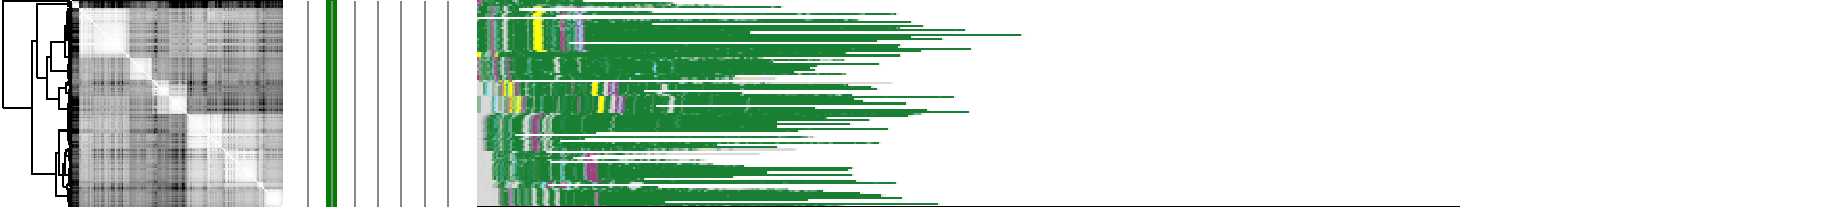
\includegraphics{haplotypes-constrained/5qtel_1-500K_1_12_12_rc-HG002.pdf}\end{textblock}
\begin{textblock}{13}(3.0,2.316)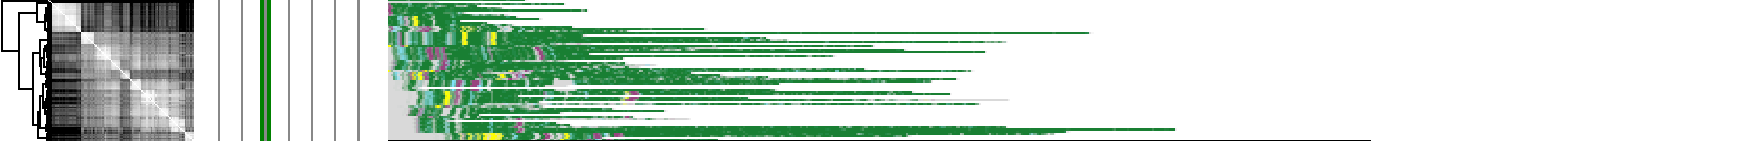
\includegraphics{haplotypes-constrained/5qtel_1-500K_1_12_12_rc-HG003.pdf}\end{textblock}
\begin{textblock}{13}(3.402799999999999,3.301)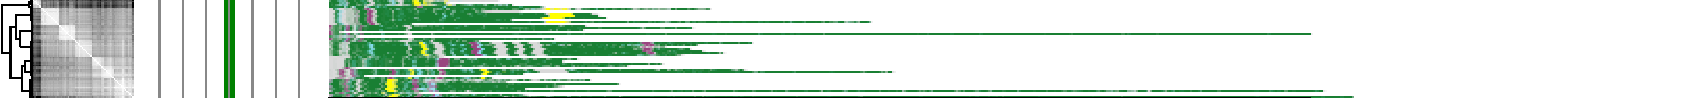
\includegraphics{haplotypes-constrained/5qtel_1-500K_1_12_12_rc-HG004.pdf}\end{textblock}
\begin{textblock}{13}(3.8610999999999986,3.993)
\includegraphics{haplotypes-constrained/5qtel_1-500K_1_12_12_rc-HG005.pdf}\end{textblock}
\begin{textblock}{13}(3.5555999999999983,4.353)
\includegraphics{haplotypes-constrained/5qtel_1-500K_1_12_12_rc-HG006.pdf}\end{textblock}
\begin{textblock}{13}(3.027799999999999,4.934)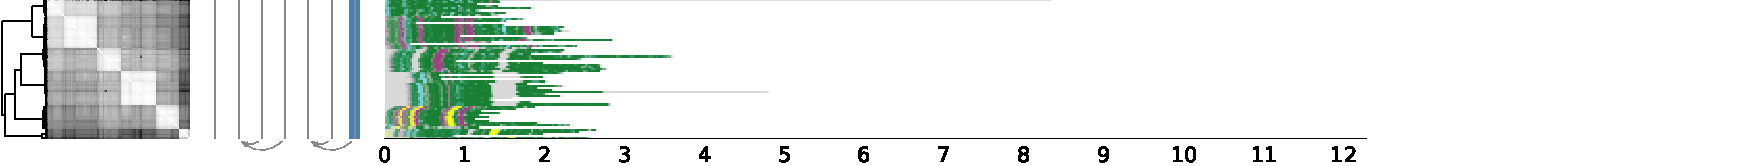
\includegraphics{haplotypes-constrained/5qtel_1-500K_1_12_12_rc-HG007.pdf}\end{textblock}
\begin{textblock}{13}(3.7360999999999986,6.126)
\includegraphics{haplotypes-constrained/6qtel_1-500K_1_12_12_rc-HG001.pdf}\end{textblock}
\begin{textblock}{13}(2.7916999999999987,6.568)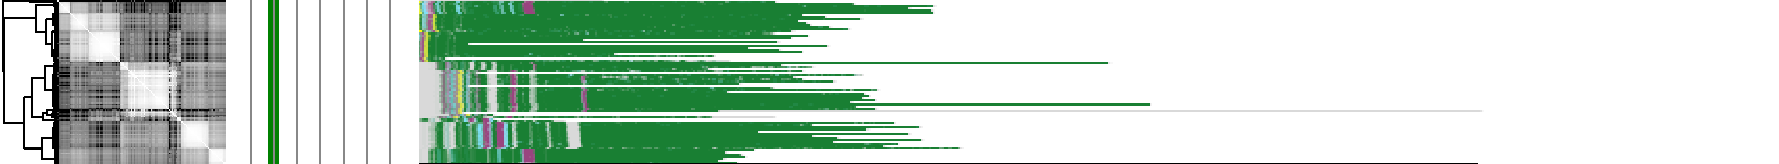
\includegraphics{haplotypes-constrained/6qtel_1-500K_1_12_12_rc-HG002.pdf}\end{textblock}
\begin{textblock}{13}(3.7083999999999993,7.706)
\includegraphics{haplotypes-constrained/6qtel_1-500K_1_12_12_rc-HG003.pdf}\end{textblock}
\begin{textblock}{13}(3.7360999999999986,8.176)
\includegraphics{haplotypes-constrained/6qtel_1-500K_1_12_12_rc-HG004.pdf}\end{textblock}
\begin{textblock}{13}(3.8055999999999983,8.619)
\includegraphics{haplotypes-constrained/6qtel_1-500K_1_12_12_rc-HG005.pdf}\end{textblock}
\begin{textblock}{13}(3.6805999999999983,9.006)
\includegraphics{haplotypes-constrained/6qtel_1-500K_1_12_12_rc-HG006.pdf}\end{textblock}
\begin{textblock}{13}(3.6805999999999983,9.491)
\includegraphics{haplotypes-constrained/6qtel_1-500K_1_12_12_rc-HG007.pdf}\end{textblock}
\begin{textblock}{13}(4.055599999999998,10.196)
\includegraphics{haplotypes-constrained/chr7-HG001.pdf}\end{textblock}
\begin{textblock}{13}(3.402799999999999,10.402)
\includegraphics{haplotypes-constrained/chr7-HG002.pdf}\end{textblock}
\begin{textblock}{13}(3.9583999999999993,11.095)
\includegraphics{haplotypes-constrained/chr7-HG003.pdf}\end{textblock}
\begin{textblock}{13}(4.027799999999999,11.385)
\includegraphics{haplotypes-constrained/chr7-HG004.pdf}\end{textblock}
\begin{textblock}{13}(4.097199999999999,11.619)
\includegraphics{haplotypes-constrained/chr7-HG005.pdf}\end{textblock}
\begin{textblock}{13}(4.0139,11.798)
\includegraphics{haplotypes-constrained/chr7-HG006.pdf}\end{textblock}
\begin{textblock}{13}(3.9860999999999986,12.047)
\includegraphics{haplotypes-constrained/chr7-HG007.pdf}\end{textblock}
\begin{textblock}{13}(4.027799999999999,12.529)
\includegraphics{haplotypes-constrained/chr8-HG001.pdf}\end{textblock}
\begin{textblock}{13}(3.375,12.764)
\includegraphics{haplotypes-constrained/chr8-HG002.pdf}\end{textblock}
\begin{textblock}{13}(3.902799999999999,13.471)
\includegraphics{haplotypes-constrained/chr8-HG003.pdf}\end{textblock}
\begin{textblock}{13}(4.027799999999999,13.802)
\includegraphics{haplotypes-constrained/chr8-HG004.pdf}\end{textblock}
\begin{textblock}{13}(4.041699999999999,14.037)
\includegraphics{haplotypes-constrained/chr8-HG005.pdf}\end{textblock}
\begin{textblock}{13}(4.027799999999999,14.257)
\includegraphics{haplotypes-constrained/chr8-HG006.pdf}\end{textblock}
\begin{textblock}{13}(3.8194999999999997,14.492)
\includegraphics{haplotypes-constrained/chr8-HG007.pdf}\end{textblock}
\begin{textblock}{13}(4.0,15.099)
\includegraphics{haplotypes-constrained/chr11-HG001.pdf}\end{textblock}
\begin{textblock}{13}(3.5138999999999996,15.362)
\includegraphics{haplotypes-constrained/chr11-HG002.pdf}\end{textblock}
\begin{textblock}{13}(3.8610999999999986,15.971)
\includegraphics{haplotypes-constrained/chr11-HG003.pdf}\end{textblock}
\begin{textblock}{13}(4.041699999999999,16.331)
\includegraphics{haplotypes-constrained/chr11-HG004.pdf}\end{textblock}
\begin{textblock}{13}(4.097199999999999,16.551)
\includegraphics{haplotypes-constrained/chr11-HG005.pdf}\end{textblock}
\begin{textblock}{13}(4.0139,16.730)
\includegraphics{haplotypes-constrained/chr11-HG006.pdf}\end{textblock}
\begin{textblock}{13}(3.6805999999999983,16.978)
\includegraphics{haplotypes-constrained/chr11-HG007.pdf}\end{textblock}
\begin{textblock}{13}(4.055599999999998,17.697)
\includegraphics{haplotypes-constrained/chr12-HG001.pdf}\end{textblock}
\begin{textblock}{13}(3.5694999999999997,17.904)
\includegraphics{haplotypes-constrained/chr12-HG002.pdf}\end{textblock}
\begin{textblock}{13}(3.722199999999999,18.472)
\includegraphics{haplotypes-constrained/chr12-HG003.pdf}\end{textblock}
\begin{textblock}{13}(3.9583999999999993,18.928)
\includegraphics{haplotypes-constrained/chr12-HG004.pdf}\end{textblock}
\begin{textblock}{13}(4.041699999999999,19.218)
\includegraphics{haplotypes-constrained/chr12-HG005.pdf}\end{textblock}
\begin{textblock}{13}(4.0695,19.439)
\includegraphics{haplotypes-constrained/chr12-HG006.pdf}\end{textblock}
\begin{textblock}{13}(4.125,19.646)
\includegraphics{haplotypes-constrained/chr12-HG007.pdf}\end{textblock}
\begin{textblock}{13}(4.125,20.031)
\includegraphics{haplotypes-constrained/14qtel_1-500K_1_12_12_rc-HG001.pdf}\end{textblock}
\begin{textblock}{13}(3.4583999999999993,20.196)
\includegraphics{haplotypes-constrained/14qtel_1-500K_1_12_12_rc-HG002.pdf}\end{textblock}
\begin{textblock}{13}(3.9166999999999987,20.847)
\includegraphics{haplotypes-constrained/14qtel_1-500K_1_12_12_rc-HG003.pdf}\end{textblock}
\begin{textblock}{13}(4.152799999999999,21.165)
\includegraphics{haplotypes-constrained/14qtel_1-500K_1_12_12_rc-HG004.pdf}\end{textblock}
\begin{textblock}{13}(4.180599999999998,21.302)
\includegraphics{haplotypes-constrained/14qtel_1-500K_1_12_12_rc-HG005.pdf}\end{textblock}
\begin{textblock}{13}(4.1389,21.426)
\includegraphics{haplotypes-constrained/14qtel_1-500K_1_12_12_rc-HG006.pdf}\end{textblock}
\begin{textblock}{13}(4.1389,21.577)
\includegraphics{haplotypes-constrained/14qtel_1-500K_1_12_12_rc-HG007.pdf}\end{textblock}
\begin{textblock}{13}(3.6666999999999987,21.962)
\includegraphics{haplotypes-constrained/chr15-HG001.pdf}\end{textblock}
\begin{textblock}{13}(3.847199999999999,22.461)\includegraphics{haplotypes-constrained/chr15-HG002.pdf}\end{textblock}
\begin{textblock}{13}(3.972199999999999,22.820)\includegraphics{haplotypes-constrained/chr15-HG003.pdf}\end{textblock}
\begin{textblock}{13}(3.9166999999999987,23.096)\includegraphics{haplotypes-constrained/chr15-HG004.pdf}\end{textblock}
\begin{textblock}{13}(3.7916999999999987,23.414)\includegraphics{haplotypes-constrained/chr15-HG005.pdf}\end{textblock}
\begin{textblock}{13}(3.3055999999999983,23.829)\includegraphics{haplotypes-constrained/chr15-HG006.pdf}\end{textblock}
\begin{textblock}{13}(3.625,24.591)\includegraphics{haplotypes-constrained/chr15-HG007.pdf}\end{textblock}
\begin{textblock}{13}(4.222199999999999,25.338)\includegraphics{haplotypes-constrained/16qtel_1-500K_1_12_12_rc-HG002.pdf}\end{textblock}
\begin{textblock}{13}(4.222199999999999,25.433)\includegraphics{haplotypes-constrained/16qtel_1-500K_1_12_12_rc-HG003.pdf}\end{textblock}
\begin{textblock}{13}(4.1945,25.529)\includegraphics{haplotypes-constrained/16qtel_1-500K_1_12_12_rc-HG004.pdf}\end{textblock}
\begin{textblock}{13}(4.2639,25.638)\includegraphics{haplotypes-constrained/16qtel_1-500K_1_12_12_rc-HG006.pdf}\end{textblock}
\begin{textblock}{13}(4.1945,25.692)\includegraphics{haplotypes-constrained/16qtel_1-500K_1_12_12_rc-HG007.pdf}\end{textblock}
\begin{textblock}{13}(4.152799999999999,26.022)\includegraphics{haplotypes-constrained/18qtel_1-500K_1_12_12_rc-HG001.pdf}\end{textblock}
\begin{textblock}{13}(3.5833999999999993,26.159)\includegraphics{haplotypes-constrained/18qtel_1-500K_1_12_12_rc-HG002.pdf}\end{textblock}
\begin{textblock}{13}(4.027799999999999,26.713)\includegraphics{haplotypes-constrained/18qtel_1-500K_1_12_12_rc-HG003.pdf}\end{textblock}
\begin{textblock}{13}(4.152799999999999,26.948)\includegraphics{haplotypes-constrained/18qtel_1-500K_1_12_12_rc-HG004.pdf}\end{textblock}
\begin{textblock}{13}(4.180599999999998,27.085)\includegraphics{haplotypes-constrained/18qtel_1-500K_1_12_12_rc-HG005.pdf}\end{textblock}
\begin{textblock}{13}(4.0695,27.208)\includegraphics{haplotypes-constrained/18qtel_1-500K_1_12_12_rc-HG006.pdf}\end{textblock}
\begin{textblock}{13}(4.0695,27.415)\includegraphics{haplotypes-constrained/18qtel_1-500K_1_12_12_rc-HG007.pdf}\end{textblock}
\begin{textblock}{13}(4.1945,27.842)\includegraphics{haplotypes-constrained/chr19-HG001.pdf}\end{textblock}
\begin{textblock}{13}(4.1389,27.952)\includegraphics{haplotypes-constrained/chr19-HG003.pdf}\end{textblock}
\begin{textblock}{13}(4.208399999999999,28.103)\includegraphics{haplotypes-constrained/chr19-HG004.pdf}\end{textblock}
\begin{textblock}{13}(4.027799999999999,28.212)\includegraphics{haplotypes-constrained/chr19-HG005.pdf}\end{textblock}
\begin{textblock}{13}(3.972199999999999,28.447)\includegraphics{haplotypes-constrained/chr19-HG006.pdf}\end{textblock}
\begin{textblock}{13}(4.083399999999999,28.723)\includegraphics{haplotypes-constrained/chr19-HG007.pdf}\end{textblock}
\begin{textblock}{13}(3.625,29.136)\includegraphics{haplotypes-constrained/chr21-HG001.pdf}\end{textblock}
\begin{textblock}{13}(2.3610999999999986,29.662)\includegraphics{haplotypes-constrained/chr21-HG002.pdf}\end{textblock}
\begin{textblock}{13}(3.652799999999999,31.119)\includegraphics{haplotypes-constrained/chr21-HG003.pdf}\end{textblock}
\begin{textblock}{13}(3.8333999999999993,31.631)\includegraphics{haplotypes-constrained/chr21-HG004.pdf}\end{textblock}
\begin{textblock}{13}(3.652799999999999,32.004)\includegraphics{haplotypes-constrained/chr21-HG005.pdf}\end{textblock}
\begin{textblock}{13}(3.8055999999999983,32.517)\includegraphics{haplotypes-constrained/chr21-HG006.pdf}\end{textblock}
\begin{textblock}{13}(3.777799999999999,32.918)\includegraphics{haplotypes-constrained/chr21-HG007.pdf}\end{textblock}
\begin{textblock}{13}(4.236099999999999,33.567)\includegraphics{haplotypes-constrained/chr22-HG001.pdf}\end{textblock}
\begin{textblock}{13}(2.5833999999999993,33.649)\includegraphics{haplotypes-constrained/chr22-HG002.pdf}\end{textblock}
\begin{textblock}{13}(3.8888999999999996,34.939)\includegraphics{haplotypes-constrained/chr22-HG003.pdf}\end{textblock}
\begin{textblock}{13}(3.652799999999999,35.284)\includegraphics{haplotypes-constrained/chr22-HG004.pdf}\end{textblock}
\begin{textblock}{13}(4.166699999999999,35.797)\includegraphics{haplotypes-constrained/chr22-HG005.pdf}\end{textblock}
\begin{textblock}{13}(3.472199999999999,35.934)\includegraphics{haplotypes-constrained/chr22-HG006.pdf}\end{textblock}
\begin{textblock}{13}(3.5833999999999993,36.571)\includegraphics{haplotypes-constrained/chr22-HG007.pdf}\end{textblock}
\begin{textblock}{13}(3.7638999999999996,37.346)\includegraphics{haplotypes-constrained/chrX-HG001.pdf}\end{textblock}
\begin{textblock}{13}(2.972199999999999,37.774)\includegraphics{haplotypes-constrained/chrX-HG002.pdf}\end{textblock}
\begin{textblock}{13}(4.027799999999999,38.787)\includegraphics{haplotypes-constrained/chrX-HG003.pdf}\end{textblock}
\begin{textblock}{13}(4.097199999999999,39.021)\includegraphics{haplotypes-constrained/chrX-HG004.pdf}\end{textblock}
\begin{textblock}{13}(3.847199999999999,39.200)\includegraphics{haplotypes-constrained/chrX-HG005.pdf}\end{textblock}
\begin{textblock}{13}(4.0139,39.559)\includegraphics{haplotypes-constrained/chrX-HG006.pdf}\end{textblock}
\begin{textblock}{13}(3.847199999999999,39.808)\includegraphics{haplotypes-constrained/chrX-HG007.pdf}\end{textblock}
\begin{textblock}{13}(2.1666999999999987,0.32)\rotatebox{90}{\Large{-------------------------------- 5qtel\_1-500K\_1\_12\_12\_rc --------------------------------}}\end{textblock}
\begin{textblock}{13}(2.5416999999999987,6.125554000000001)\rotatebox{90}{\Large{---------------- 6qtel\_1-500K\_1\_12\_12\_rc ----------------}}\end{textblock}
\begin{textblock}{13}(3.152799999999999,10.195552000000001)\rotatebox{90}{\Large{---------------- chr7 ----------------}}\end{textblock}
\begin{textblock}{13}(3.125,12.529441)\rotatebox{90}{\Large{----------------- chr8 -----------------}}\end{textblock}
\begin{textblock}{13}(3.2638999999999996,15.099440999999999)\rotatebox{90}{\Large{----------------- chr11 -----------------}}\end{textblock}
\begin{textblock}{13}(3.3194999999999997,17.697218)\rotatebox{90}{\Large{--------------- chr12 ---------------}}\end{textblock}
\begin{textblock}{13}(3.2083999999999993,20.031108999999997)\rotatebox{90}{\Large{14qtel\_1-500K\_1\_...}}\end{textblock}
\begin{textblock}{13}(3.0555999999999983,21.962220499999997)\rotatebox{90}{\Large{------------------------- chr15 -------------------------}}\end{textblock}
\begin{textblock}{13}(3.9444999999999997,25.337775499999996)\rotatebox{90}{\Large{16q...}}\end{textblock}
\begin{textblock}{13}(3.3333999999999993,26.022219999999997)\rotatebox{90}{\Large{18qtel\_1-500K\_1...}}\end{textblock}
\begin{textblock}{13}(3.722199999999999,27.842219699999998)\rotatebox{90}{\Large{---- chr19 ----}}\end{textblock}
\begin{textblock}{13}(2.1110999999999986,29.1361075)\rotatebox{90}{\Large{---------------------------------- chr21 ----------------------------------}}\end{textblock}
\begin{textblock}{13}(2.3333999999999993,33.567220500000005)\rotatebox{90}{\Large{---------------------------- chr22 ----------------------------}}\end{textblock}
\begin{textblock}{13}(2.722199999999999,37.34555340000001)\rotatebox{90}{\Large{---------------------- chrX ----------------------}}\end{textblock}
\begin{textblock}{13}(12.928,0)
\includegraphics[width=4.500in,keepaspectratio]{haplotypes/haplotypes-legend.pdf}
\end{textblock}
\end{document}
